\subsection{Propuesta de solución}
\begin{figure}[htb]
    \centering
    \makebox[\textwidth]{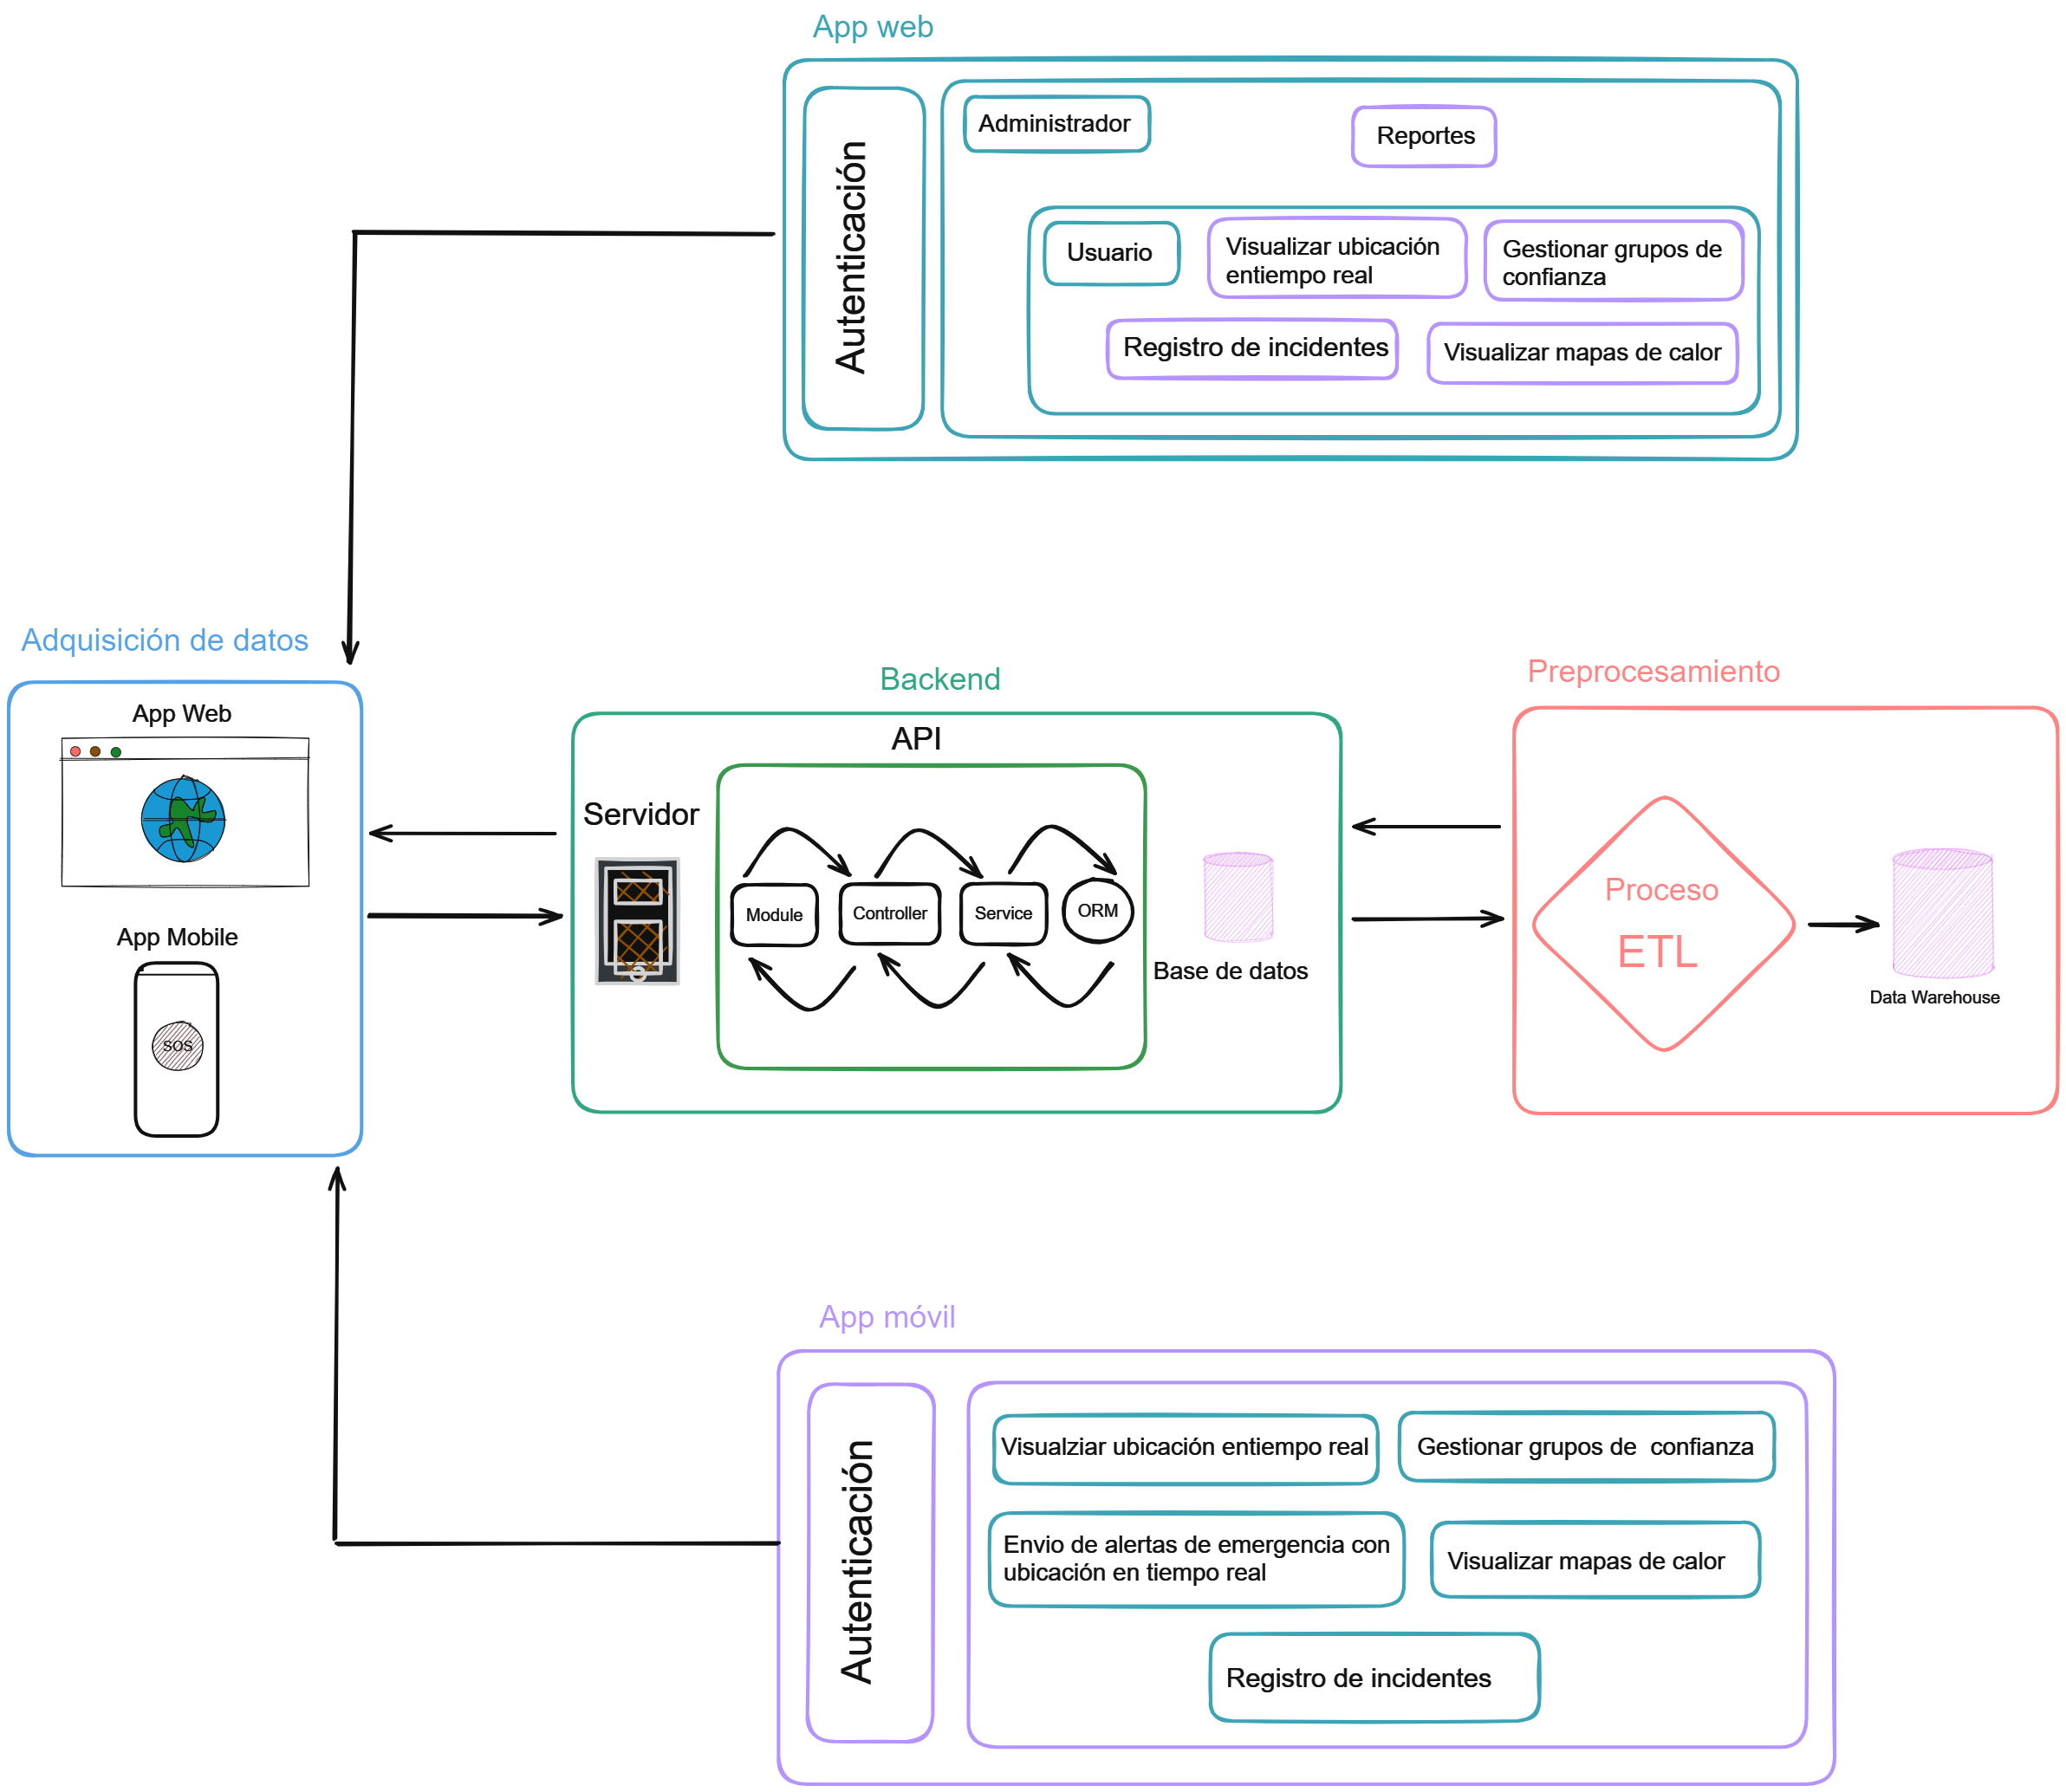
\includegraphics[width=14cm, height=12cm]{./resources/images/esquema.png}}%
    \caption{Esquema del sistema}
    \label{fig:esquema}
\end{figure}



En el proyecto propuesto para las aplicaciones cliente, se empleará una aplicación móvil, dado que esta puede ser utilizada en una gran variedad de
dispositivos, tanto Android como iOS. La aplicación móvil empleará un patrón arquitectura Model View Controller (MVC), con la cual se separará la lógica de
negocio de la interfaz de usuario y la interacción. También se utilizará un framework web, dado que este ofrece una estructura de trabajo establecida,
además de incluir características extras y optimizaciones que facilitan el desarrollo de aplicaciones web. El sistema web se desarrollará utilizando el
patrón de arquitectura MVC, dado que este permite dividir la lógica y responsabilidad en 3 capas y así mantener una mejor estructura en el código.
Para el desarrollo del backend, se emplearán frameworks que agilicen la creación de un API REST eficiente y escalable, el cual permita la comunicación
entre diferentes sistemas, como aplicaciones web y móviles, mediante el protocolo HTTP. Para el almacenamiento de información, se empleará una base de
datos relacional, dado que esta ofrece un gran rendimiento y fiabilidad al manejar grandes volúmenes de datos. Además, permite manejar relaciones entre
diferentes tablas, las cuales ayudan a recuperar datos de forma eficiente, garantizando la integridad referencial. Para el desarrollo del proyecto, se
utilizará una metodología de desarrollo ágil por la facilidad, flexibilidad y versatilidad que ofrece al realizar cambios durante el desarrollo. Además,
mejora los tiempos de desarrollo y la calidad del producto final.

\bigbreak
En concordancia con lo mencionado anteriormente, se propone el desarrollo de una aplicación móvil dedicada
a recopilar datos georreferenciados sobre delitos, mediante alertas de emergencia con ubicación en tiempo
real. Se integrarán formularios para obtener detalles de incidentes pasados. La aplicación también administrará
grupos de confianza, permitiendo el monitoreo en tiempo real de la ubicación de familiares en situaciones de
riesgo y la visualización de mapas que identifiquen zonas conflictivas. Además, se planifica una aplicación
web complementaria para visualizar en tiempo real familiares en peligro, registrar incidentes y visualizar
mapas de calor que indiquen áreas de alta incidencia delictiva. La aplicación web incluirá un sistema de roles,
otorgando al administrador acceso a reportes detallados sobre los siniestros reportados. Ambas aplicaciones
estarán interconectadas a través de un servidor que proporcionará una API REST vinculada a una base de datos
relacional. La información recolectada en esta base de datos pasará por un proceso de Extracción, Transformación
y Carga de datos (ETL) para generar un almacén de datos (data warehouse) y, posteriormente, un cubo OLAP.
Este cubo OLAP será la fuente principal de información para la generación de reportes detallados sobre la
incidencia delictiva.

\bigbreak
En este contexto, el presente proyecto de investigación es técnicamente viable, ya que se cuenta con las
herramientas necesarias para su desarrollo, así como con los conocimientos requeridos adquiridos a lo largo
de la trayectoria académica. Desde la perspectiva operativa, el proyecto es factible, ya que se dispone del
personal necesario para su ejecución, representado por los propios usuarios del sistema, quienes son ciudadanos
de Ambato. Desde el punto de vista económico, el proyecto es viable, dado que el investigador cuenta con los
recursos necesarios para asumir los costos de la investigación, asegurando la independencia financiera al
no depender de fuentes externas.